\documentclass[12pt]{article}
\usepackage[margin=0.79in]{geometry}
\usepackage{float}
\usepackage{graphicx}
\usepackage{amsmath}
\usepackage{amssymb}
\usepackage{framed}
\usepackage{subfig}
\usepackage{mathtools}
\usepackage{scrextend}
\mathtoolsset{showonlyrefs} 

\setcounter{tocdepth}{1}

\newcommand\defeq{\stackrel{\mathclap{def}}{=}}
\newcommand{\R}{\mathbb{R}}

\usepackage{listings}
\usepackage{color}

\definecolor{dkgreen}{rgb}{0,0.6,0}
\definecolor{gray}{rgb}{0.5,0.5,0.5}
\definecolor{mauve}{rgb}{0.58,0,0.82}

\lstset{frame=tb,
  language=Java,
  aboveskip=3mm,
  belowskip=3mm,
  showstringspaces=false,
  columns=flexible,
  basicstyle={\small\ttfamily},
  numbers=none,
  numberstyle=\tiny\color{gray},
  keywordstyle=\color{blue},
  commentstyle=\color{dkgreen},
  stringstyle=\color{mauve},
  breaklines=true,
  breakatwhitespace=true,
  tabsize=3
}

\begin{document}

	\title{Restoring a Blurry Image\\
		\large MTH 410, F18}
	\author{Michael Sieviec}
	\maketitle
	\tableofcontents

\begin{flushleft}
\section{Background}
Tikhonov regularization is a process for approximating \textbf{x}  as a solution to the least squares optimization problem

\begin{equation}
\min_{\widetilde{\textbf{x}} \in \R^n} f(\widetilde{\textbf{x}}), \quad \text{where} \quad 
f(\widetilde{\textbf{x}}) \defeq \|\widetilde{\textbf{d}} - \textbf{A}\widetilde{\textbf{x}}\|^2 + \lambda^2\|\widetilde{\textbf{x}}\|^2
\label{eq1}
\end{equation}

with $\widetilde{\textbf{x}}$ being found as the solution to the linear system

\begin{equation}
	(\textbf{A}^T\textbf{A} + \lambda^2\textbf{I})\widetilde{\textbf{x}}_\lambda = \textbf{A}^T\widetilde{\textbf{d}}
	\label{eq2}
\end{equation}

The following algorithm produces the desired $\widetilde{\textbf{x}}$:
\linebreak

\quad \text{Given \textbf{A}, $\widetilde{\textbf{D}}$, $\lambda$;}\\
	\quad \quad $for\:i = 1:m$ \\
	\quad \qquad$ \widetilde{\textbf{d}} = \widetilde{\textbf{D}}(:,i)$ \quad \% column $i$ of the noisy data matrix $\widetilde{\textbf{D}}$\\
	\quad \qquad evaluate $\widetilde{\textbf{x}}_i$ by solving \eqref{eq2}\\
	\quad \quad $end$
\linebreak
\linebreak
Compiling $\widetilde{\textbf{X}}_\lambda = [\widetilde{\textbf{x}}_1 \: \widetilde{\textbf{x}}_2 \dots \widetilde{\textbf{x}}_m]$ yields the solution matrix $\widetilde{\textbf{X}}_\lambda \approx \textbf{X}$, where \textbf{X} is the original, undistorted matrix.

\section{Application}

One area of use for Tikhonov regularization is image restoration. Observe the following blurred image of a US dollar bill:

\begin{figure}[H]
	\centering
	\captionsetup{justification=centering}
	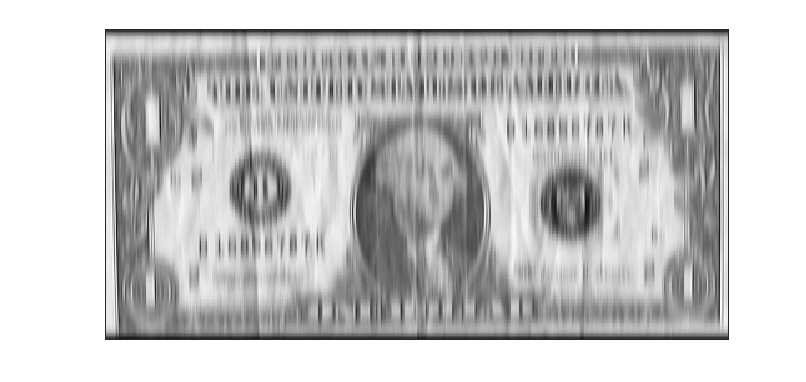
\includegraphics[scale=0.55]{images/dollarblur.png}
	\caption{Blurred dollar bill, original}
\end{figure}
\ \\

In order to decipher the serial number on the bill, we apply Tikhonov regularization (the code for which can be found in section \ref{code}) to the image data matrix with various values of $\lambda$ until we have a reasonably clear result. Hansen \cite{hansen} found that small -- $10^{-1}$ to $10^{-5}$ -- values of $\lambda$ were appropriate for minimizing \eqref{eq1}.
\ \\
\ \\
For $\lambda  = 1$, we have

\begin{figure}[H]
	\centering
	\captionsetup{justification=centering}
	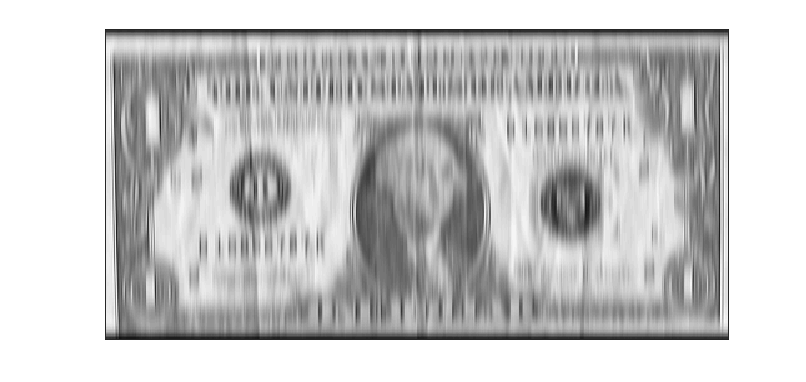
\includegraphics[scale=0.55]{images/lambda1.png}
	\caption{Blurred dollar bill, regularized, $\lambda = 1$}
\end{figure}
\ \\
The resolution of which is perhaps slightly worse than the original. $\lambda = 10^{-1}$ yields

\begin{figure}[H]
	\centering
	\captionsetup{justification=centering}
	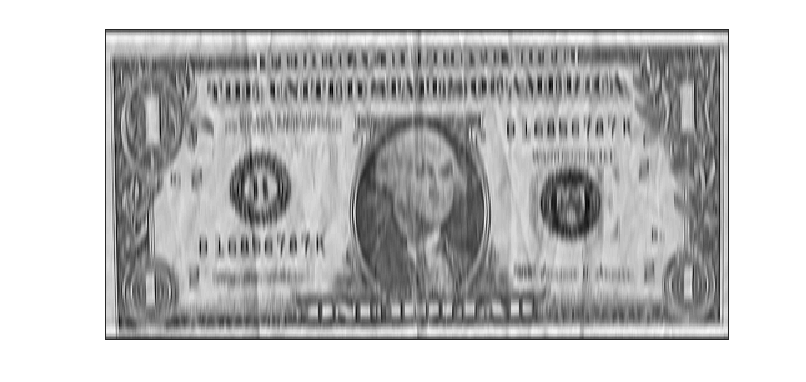
\includegraphics[scale=0.55]{images/lambda01.png}
	\caption{Blurred dollar bill, regularized, $\lambda = 10^{-1}$}
\end{figure}
\ \\
\ \\
This is significantly clearer. The next several figures show the results of further values of $\lambda$.

\begin{figure}[H]
	\centering
	\captionsetup{justification=centering}
	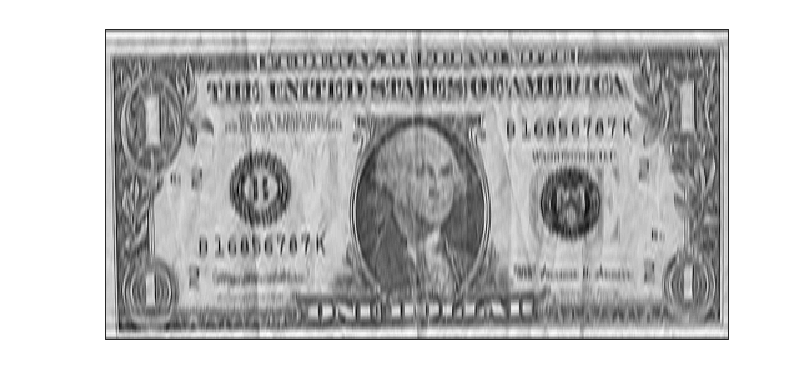
\includegraphics[scale=0.55]{images/lambda001.png}
	\caption{Blurred dollar bill, regularized, $\lambda = 10^{-2}$}
\end{figure}
\ \\

\begin{figure}[H]
	\centering
	\captionsetup{justification=centering}
	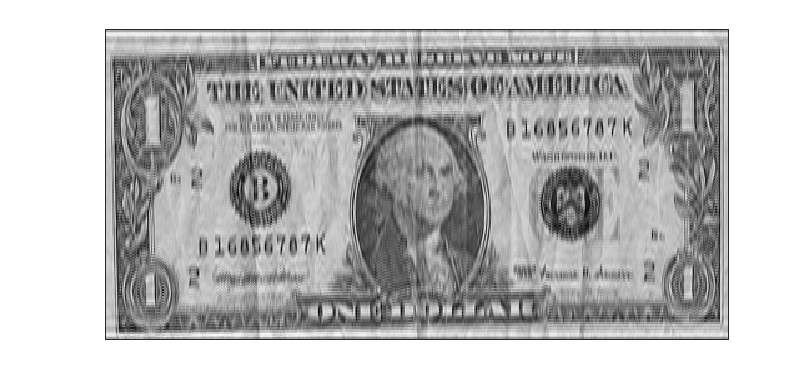
\includegraphics[scale=0.55]{images/lambda0001.png}
	\caption{Blurred dollar bill, regularized, $\lambda = 10^{-3}$}
\end{figure}
\ \\

\begin{figure}[H]
	\centering
	\captionsetup{justification=centering}
	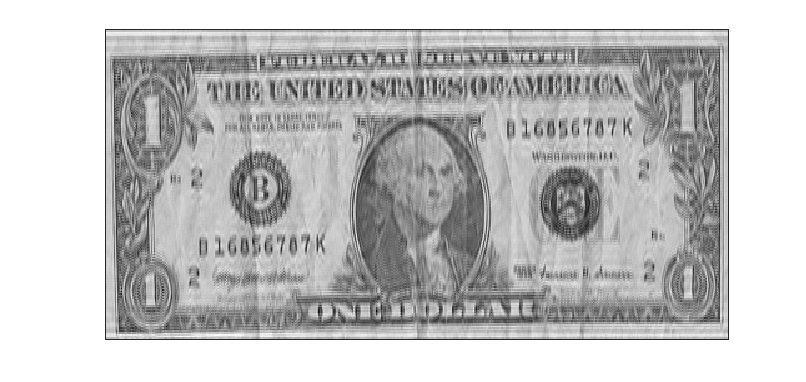
\includegraphics[scale=0.55]{images/lambda00001.png}
	\caption{Blurred dollar bill, regularized, $\lambda = 10^{-4}$}
	\label{lambda4}
\end{figure}
\ \\

\begin{figure}[H]
	\centering
	\captionsetup{justification=centering}
	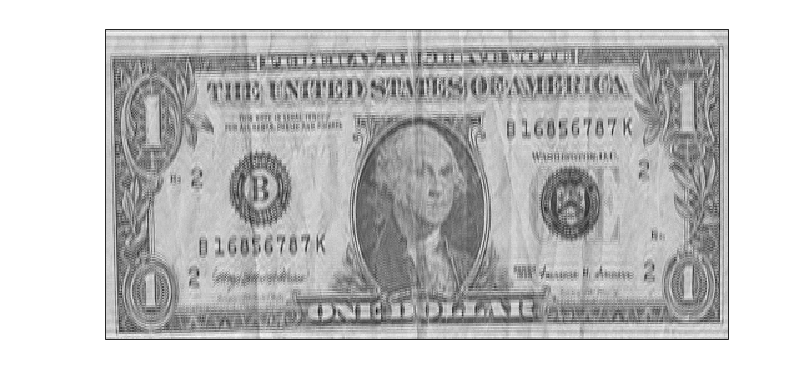
\includegraphics[scale=0.55]{images/lambda000001.png}
	\caption{Blurred dollar bill, regularized, $\lambda = 10^{-5}$}
	\label{lambda5}
\end{figure}
\ \\

\begin{figure}[H]
	\centering
	\captionsetup{justification=centering}
	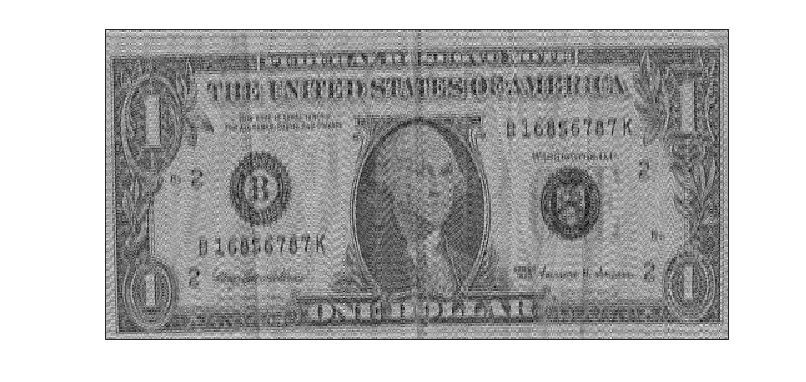
\includegraphics[scale=0.55]{images/lambda0000001.png}
	\caption{Blurred dollar bill, regularized, $\lambda = 10^{-6}$}
	\label{lambda6}
\end{figure}
\ \\
\ \\
We see that figures \ref{lambda4} and \ref{lambda5} -- $\lambda = 10^{-4}$ and $10^{-5}$, respectively -- produce the clearest serial numbers, and that as we progress into figure \ref{lambda6}, $\lambda = 10^{-6}$, we introduce more noise into the solution norm, obscuring the picture again.
\ \\
\ \\
Based on the results, the serial number appears to be D16856787K, meaning it was manufactured in Cleveland \cite{serial}. However, due to the lack of total clarity, it is possible for the D to be a B and for it to have been manufactured in New York.

\section{Code} \label{code}

\begin{lstlisting}[language=Matlab]
function Xapp = tikhonov(lambda,Dapp)

% This function uses Tikhonov regularization to approximate an original
% matrix from a given noisy matrix.

% lambda    - regularization parameter    
% Dapp      - noisy data matrix

[Dm,Dn] = size(Dapp); % size constraints for function
L = 0.45; % given parameter

% create B, A, I matrices

B = zeros(Dm,Dm);

for i = 1:Dm
    B(i,i) = 1 - 2*L;
    if (i <= Dm-1)
        B(i,i+1) = L;
        B(i+1,i) = L;
    end
end

A = B^25; % non-singular transformation matrix
I = eye(size(A)); % Dm x Dm identity matrix

% solve approximate X original matrix

for j = 1:Dn
    d = Dapp(:,j);
    x = (A'*A + lambda^2*I)\A'*d;
    Xapp(:,j) = x;
end

end
\end{lstlisting}

\begin{thebibliography}{1}
\bibitem{hansen}
Hansen, P.C. (2000). "The L-curve and its use in the numerical treatment of inverse problems." 3. https://www.sintef.no/globalassets/project/evitameeting/2005/lcurve.pdf (accessed November 21, 2018).

\bibitem{serial}
U.S. Bureau of Engraving and Printing. "Federal Reserve Bank and Serial Number Relationship Table." MoneyFactory.gov. https://www.moneyfactory.gov/frbsntable.html (accessed November 21, 2018).
\end{thebibliography}

\end{flushleft}
\end{document}